\documentclass[11pt, a4paper]{article}

% --- Packages ---
\usepackage[utf8]{inputenc}
\usepackage[T1]{fontenc}
\usepackage{mathptmx} % Times New Roman font for professional document typography
\usepackage{graphicx}
\usepackage[margin=0.8in]{geometry}
\usepackage{xcolor}
\usepackage{titlesec}
\usepackage{enumitem}
\usepackage{float}
\usepackage{booktabs}
\usepackage{multirow}
\usepackage{array}
\usepackage{url}

% --- Amrita Colors ---
\definecolor{amritaMaroon}{HTML}{A4123F}

% --- Title & Section Formatting ---
\titlespacing*{\section}{0pt}{12pt}{4pt}
\titlespacing*{\subsection}{0pt}{8pt}{3pt}
\titleformat{\section}{\large\bfseries\color{amritaMaroon}}{\thesection}{0.8em}{}
\titleformat{\subsection}{\normalsize\bfseries\color{amritaMaroon}}{\thesubsection}{0.6em}{}

\pagestyle{plain}

\begin{document}

% ==========================================
% HEADER & TITLE BLOCK
% ==========================================
\noindent
\begin{minipage}{\textwidth}
    \centering
    {\Large \textbf{\textcolor{amritaMaroon}{
    AMRITA VISHWA VIDYAPEETHAM \\
    SCHOOL OF COMPUTING \\
    DEPARTMENT OF COMPUTER SCIENCE AND ENGINEERING \\
    }}}
    \vspace{0.2cm}
    {\large \textbf{NEXUS-Foundry: A Cross-Stage Cognitive Digital Twin Platform for Predictive Casting Intelligence}} \\[0.1cm]
    \textbf{23CSE498 -- Project Phase II (External Review)} \quad | \quad \textbf{Team Number: G016} \\
    \today
\end{minipage}

\vspace{0.3cm}
\hrule
\vspace{0.3cm}

% --- Team & Guide Details ---
\noindent
\begin{center}
    \renewcommand{\arraystretch}{1.45}
    \setlength{\tabcolsep}{6pt}
    \begin{tabular}{|l|p{4.8cm}|p{4.6cm}|p{3.2cm}|}
        \hline
        \multicolumn{2}{|c|}{\textbf{Team Members}} & \textbf{Project Guide} & \textbf{Project Type} \\
        \hline
        \small CB.SC.U4CSE23150 & \small \raggedright Subiksha M.V &
        \multirow{4}{=}{\raggedright \small \textbf{Dr. Bagavathi Sivakumar P.} \newline \textit{Chairperson, \newline Dept. of CSE}} &
        \multirow{4}{=}{\raggedright \small \textbf{Type 3} \newline Software-Based Project} \\ \cline{1-2}
        \small CB.SC.U4CSE23516 & \small C.B. Harinie & & \\ \cline{1-2}
        \small CB.SC.U4CSE23520 & \small K. Kanishthika & & \\ \cline{1-2}
        \small CB.SC.U4CSE23542 & \small P. Pon Gopika & & \\
        \hline
    \end{tabular}
\end{center}
\vspace{0.2cm}

% --- 1. ABSTRACT ---
\section{Abstract}
\noindent
High-temperature metal casting operations (1350$^\circ$C to 1560$^\circ$C) in gray iron (ASTM A48) and ductile iron (ASTM A536) foundries are severely encumbered by process fragmentation across melting, molding, pouring, and visual inspection stages. Because operational deviations at the furnace propagate invisibly downstream, casting defects such as gas porosity, cold shuts, and micro-shrinkage are typically discovered 15+ hours after casting, resulting in 8\%--15\% scrap rates and catastrophic refractory wear. NEXUS-Foundry solves this challenge through an end-to-end, event-driven cyber-physical digital twin platform that connects all four foundry stages into a closed-loop intelligence system. In Phase II, complete (100\%) software integration has been achieved across a 7-layer architecture encompassing an asynchronous FastAPI gateway, four stateful digital twins with Redis state caching, a polyglot persistence tier (InfluxDB and PostgreSQL), and an interactive React 18 Three.js/R3F operator dashboard. The platform embeds a 6-tier hybrid machine learning suite comprising an LSTM Autoencoder (LSTM-AE) for sub-35ms furnace anomaly detection, a Temporal Fusion Transformer (TFT) for 48-hour multi-quantile degradation forecasting ($R^2 = 0.982$, $\text{MAE} = 12.4^\circ\text{C}$), an XGBoost pre-pour defect classifier ($\text{ROC-AUC} = 0.968$), TreeSHAP for real-time feature explainability ($<10\text{ ms}$), a Physics-Informed Neural Network (PINN) simulating Fourier heat conduction ($<25\text{ ms}$), and a triple-grounded RAG cognitive assistant. Comprehensive unit, integration, and full-stream replay testing on 739k+ telemetry records validate that upstream furnace excursions dispatch automated cross-stage alerts in $<2.0\text{ seconds}$, mitigating defect risks before molten metal enters the mold.

% --- 2. SOFTWARE REQUIREMENTS SPECIFICATION (SRS) ---
\section{Software Requirements Specification (SRS)}

\subsection{Product Scope, Actors \& Use Cases}
\begin{itemize}[noitemsep, topsep=2pt]
    \item \textbf{Software Purpose \& Scope:} NEXUS-Foundry provides an industrial-grade cyber-physical digital twin and AI decision-support platform designed for green sand casting foundries. Its operational boundary covers real-time shop-floor sensor ingestion (MQTT/Kafka), synchronized digital twin state tracking, cross-stage anomaly cascading, pre-pour defect risk evaluation, physics-constrained simulation, and continuous model retraining.
    \item \textbf{User Roles / Actors:} 
    \textit{Furnace Operator} (monitors crucible melt temperatures, coil vibration, power draw, and receives acoustic/visual anomaly warnings); 
    \textit{Process Engineer} (analyzes green sand conditioning parameters, evaluates TreeSHAP risk attributions, and executes PINN what-if simulations); 
    \textit{Quality Inspector} (reviews optical surface classification outputs and inputs verified ground-truth labels); 
    \textit{Plant Supervisor} (tracks active batch timelines, overall scrap rates, and energy tariff schedules); 
    \textit{Automated Background Worker} (ingests sensor streams and retrains models upon label queue accumulation).
    \item \textbf{Comparison with Existing Systems:} Conventional furnace systems (e.g., Ipsen PdMetrics) monitor equipment health in isolation but lack downstream quality foresight \cite{vijaykumar2025}. Standalone visual inspection tools (e.g., Allus AI) classify defects with high precision but only post-solidification, resulting in irreversible material and energy waste. General factory visualization suites (e.g., Siemens Digital Twin Composer) provide 3D layouts but lack foundry-specific pyrometallurgical kinetics and thermodynamic PDE constraints \cite{vanwyk2024, zhou2025}. NEXUS-Foundry bridges this gap by unifying cross-stage propagation with physics-grounded AI.
    \item \textbf{Core Use Cases:}
    \begin{enumerate}[noitemsep, topsep=2pt]
        \item \textbf{UC-01 (Furnace Anomaly Detection \& Degradation Forecasting):} \textit{Actor:} Furnace Operator. \textit{Precondition:} Coreless induction furnace sensor stream active at 2-second cadence. \textit{Main Flow:} Telemetry is ingested by the Melting Twin; LSTM-AE evaluates sliding 30-step windows; if reconstruction MSE exceeds $\tau = 0.78$, an anomaly event triggers an emergency TFT run returning 48-hour $P10/P50/P90$ quantile forecasts. \textit{Postcondition:} Millisecond-timestamped critical alert is rendered and cross-stage warning is dispatched.
        \item \textbf{UC-02 (Cross-Stage Pre-Pour Defect Risk Evaluation):} \textit{Actor:} Process Engineer. \textit{Precondition:} Active batch scheduled for pouring within 12 hours. \textit{Main Flow:} Pouring Twin receives upstream anomaly notification ($<2.0\text{ s}$); queries Molding Twin for sand moisture and permeability; extracts 50-dimensional CAD shape embeddings; builds a standardized 65-feature vector; executes XGBoost and TreeSHAP. \textit{Postcondition:} Pre-pour risk score (PASS vs. HIGH\_RISK) and exact feature attribution percentages are surfaced to the operator before metal enters the mold.
        \item \textbf{UC-03 (Physics-Informed What-If Simulation Sandbox):} \textit{Actor:} Plant Supervisor / Process Engineer. \textit{Precondition:} Defect risk elevated on scheduled batch. \textit{Main Flow:} Operator adjusts hypothetical setpoints (power trim, pour speed, moisture) in the PINN Sandbox; PINN evaluates 2D transient thermal conduction ($\frac{\partial T}{\partial t} = \alpha \nabla^2 T$); returns cooling rate and physical validity in $<25\text{ ms}$. \textit{Postcondition:} Thermodynamically consistent setpoints are confirmed, reducing defect probability without shop-floor trial and error.
    \end{enumerate}
\end{itemize}

\subsection{Functional \& Non-Functional Requirements}
\begin{table}[H]
    \centering
    \footnotesize
    \renewcommand{\arraystretch}{1.25}
    \begin{tabular}{|c|p{2.8cm}|p{9.4cm}|}
        \hline
        \textbf{Req. ID} & \textbf{Category} & \textbf{Requirement Specification} \\
        \hline
        {[FR-01]} & Data Acquisition & Ingest high-frequency multi-stage sensor streams via MQTT and Kafka at 2-second sampling intervals with schema validation. \\
        \hline
        {[FR-02]} & Digital Twin State & Maintain four stateful virtual twins (Melting, Molding, Pouring, Quality) with Redis hot-caching and persistent state recovery. \\
        \hline
        {[FR-03]} & Anomaly Detection & Execute unsupervised LSTM Autoencoder inference every 2 seconds; flag critical warnings when reconstruction MSE exceeds $\tau = 0.78$. \\
        \hline
        {[FR-04]} & Multi-Horizon Forecast & Execute Temporal Fusion Transformer (TFT) generating 48-hour degradation projections with $P10$, $P50$, and $P90$ confidence intervals. \\
        \hline
        {[FR-05]} & Pre-Pour Defect Risk & Assemble standardized 65-dimensional vectors (process + chemistry + CAD geometry) to predict defect risk via XGBoost with TreeSHAP attributions. \\
        \hline
        {[FR-06]} & Physics Simulation & Simulate 2D transient thermal fields using a PyTorch PINN constrained by Fourier's law; validate cooling rates in $<3.0\text{ seconds}$. \\
        \hline
        {[FR-07]} & Continuous Retraining & Buffer verified human inspection labels in a Redis training queue; trigger automated background model retraining upon reaching 50 samples. \\
        \hline
        {[NFR-01]} & Performance \& Latency & End-to-end pipeline latency (sensor $\rightarrow$ twin $\rightarrow$ dashboard) must not exceed 2.0 seconds; model inference latencies: LSTM-AE $<35\text{ ms}$, XGBoost $<5\text{ ms}$, SHAP $<10\text{ ms}$. \\
        \hline
        {[NFR-02]} & Availability \& Recovery & Achieve $>99.5\%$ operational uptime; containerized twin state must be fully restorable from persistent storage within 30 seconds of service restart. \\
        \hline
        {[NFR-03]} & Security \& Privacy & Deploy 100\% on-premise inference with local Llama 3 via Ollama; enforce role-based access control (RBAC), 8-hour token expiry, and Docker network isolation. \\
        \hline
        {[NFR-04]} & Explainability & Every defect prediction must provide decomposed game-theoretic SHAP feature attributions across temperature, lining, sand, and geometry groups. \\
        \hline
    \end{tabular}
    \caption{Software Functional and Non-Functional Requirements Specification}
\end{table}

% --- 3. SOFTWARE ARCHITECTURE & SYSTEM DESIGN ---
\section{Software Architecture \& System Design}

\subsection{High-Level System Architecture}
\noindent
NEXUS-Foundry is architected as an event-driven, 7-layer cyber-physical system. Sensor telemetry generated by optical pyrometers, accelerometers, power current transformers, and mold sensors is ingested via Eclipse Mosquitto (MQTT) and buffered into Apache Kafka topics. An asynchronous FastAPI gateway consumes these events, persists raw time-series points into InfluxDB, and routes updates to the corresponding Digital Twin service. Each digital twin (Melting, Molding, Pouring, Quality) maintains its state in an in-memory state machine backed by Redis. Anomaly events trigger the analytics layer (LSTM-AE, TFT, XGBoost, TreeSHAP, and PINN), which in turn broadcasts state updates and audit traces over a WebSocket channel to the React 18 / Three.js operator interface.

\begin{figure}[H]
    \centering
    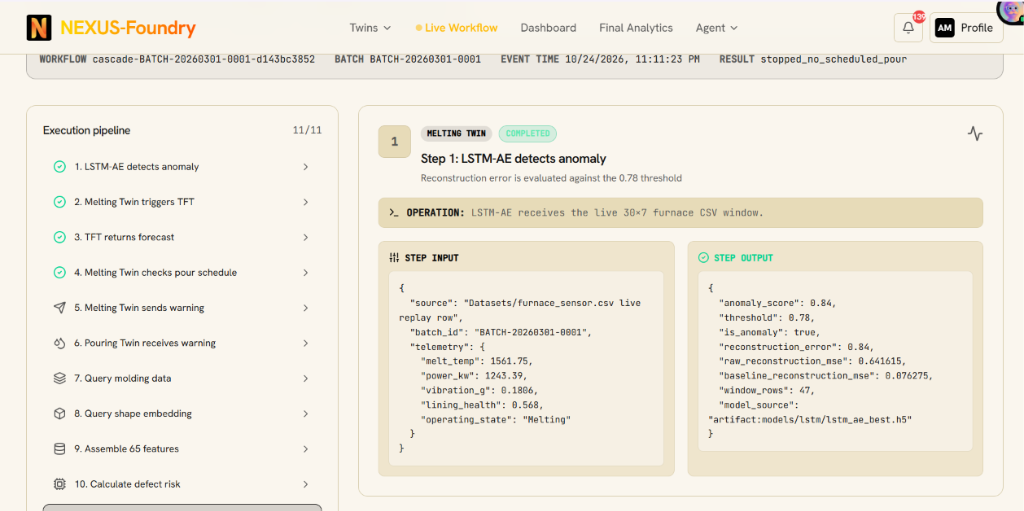
\includegraphics[width=0.95\textwidth]{docs/screenshots/04_live_workflow_execution_pipeline.png}
    \caption{High-Level Software System Architecture: End-to-End Cross-Stage Execution and Audit Pipeline}
\end{figure}

\subsection{Database Schema \& Data Modeling}
\noindent
The persistence architecture adopts a polyglot storage model optimized for distinct industrial access patterns:
(1) \textbf{InfluxDB 2.7} stores time-series sensor points under the \texttt{sensor\_readings} bucket, indexed by tags (\texttt{batch\_id}, \texttt{furnace\_id}, \texttt{ladle\_id}, \texttt{stage}) with high-precision timestamps for rapid rolling window calculations;
(2) \textbf{PostgreSQL 15} manages relational production entities including \texttt{batches} (\texttt{batch\_id} PK, \texttt{alloy\_grade}, \texttt{target\_temp}, \texttt{pour\_time}), \texttt{geometries} (\texttt{geometry\_id} PK, \texttt{part\_name}, \texttt{surface\_volume\_ratio}, \texttt{shape\_embedding} vector[50]), \texttt{materials} (\texttt{grade} PK, thermal diffusivity, conductivity), and \texttt{inspection\_labels};
(3) \textbf{Redis 7} acts as a low-latency key-value cache holding active twin snapshots (\texttt{twin:melting:state}) and the FIFO retraining queue;
(4) \textbf{ChromaDB} stores 384-dimensional vector embeddings of AFS casting handbooks and ASTM standards for the RAG cognitive assistant.

\begin{figure}[H]
    \centering
    \fbox{\begin{minipage}[c][4.4cm]{0.95\textwidth}
        \centering
        \textbf{NEXUS-Foundry Polyglot Data Model \& Storage Hierarchy} \\[0.25cm]
        \footnotesize
        \begin{tabular}{|p{3.2cm}|p{3.8cm}|p{4.2cm}|p{2.4cm}|}
            \hline
            \textbf{Store \& Engine} & \textbf{Primary Entity / Bucket} & \textbf{Key Schema Attributes} & \textbf{Access Pattern} \\
            \hline
            \textbf{InfluxDB 2.7} (TSDB) & \texttt{sensor\_readings} & \texttt{time}, \texttt{batch\_id}, \texttt{melt\_temp}, \texttt{power\_kw}, \texttt{vibration\_g} & Append-heavy, 2s sliding window queries \\
            \hline
            \textbf{PostgreSQL 15} (Relational) & \texttt{batches}, \texttt{geometries}, \texttt{inspection\_labels} & \texttt{batch\_id} PK, \texttt{shape\_embedding} [50], \texttt{defect\_type}, \texttt{severity} & ACID transactions, relational batch joins \\
            \hline
            \textbf{Redis 7} (Key-Value) & \texttt{twin:\{stage\}:state}, \texttt{retraining\_queue} & JSON serialized twin states, FIFO queue for verified inspection labels & Sub-millisecond reads, Pub/Sub cache \\
            \hline
            \textbf{ChromaDB} (Vector Store) & \texttt{foundry\_manuals} & Document chunks, 384-dim sentence embeddings, metadata & Cosine similarity k-NN vector retrieval \\
            \hline
        \end{tabular}
    \end{minipage}}
    \caption{Database Schema and Polyglot Data Model Design}
\end{figure}

\subsection{Subsystem Decomposition \& API Contracts}
\begin{table}[H]
    \centering
    \footnotesize
    \renewcommand{\arraystretch}{1.25}
    \begin{tabular}{|p{3.6cm}|p{3.8cm}|p{6.2cm}|}
        \hline
        \textbf{Interface / Endpoint} & \textbf{Subsystem / Module} & \textbf{Purpose, Request Payload \& Response Contract} \\
        \hline
        \texttt{GET /api/v1/digital-twins/\{twin\}/state} & Digital Twin Subsystem & Fetches current state snapshot of specified twin. \newline \textbf{Output:} JSON object containing live sensor values, operating state, anomaly scores, and ISO timestamp. \\
        \hline
        \texttt{WS /ws} & Real-Time Broadcast & Full-duplex WebSocket stream. Transmits synchronized state updates across all four twins to connected operator cockpits every 2s. \\
        \hline
        \texttt{POST /api/v1/simulation/what-if} & PINN Physics Sandbox & Evaluates thermodynamic validity of parameter trims. \newline \textbf{Input:} \texttt{\{"twin": "pouring", "parameters": \{...\}\}} \newline \textbf{Output:} Predicted state, cooling rate, solidification time, physical validity boolean, and operational guidance. \\
        \hline
        \texttt{GET /api/v1/workflows/cascade} & Cross-Stage Workflow Engine & Retrieves execution audit trail for active anomaly cascade. \newline \textbf{Output:} Ordered list of 11 pipeline steps with verified execution latency and input/output JSON contracts. \\
        \hline
        \texttt{POST /api/v1/chat} & RAG Cognitive Copilot & Answers natural-language operator queries. \newline \textbf{Input:} \texttt{\{"message": "...", "batch\_id": "..."\}} \newline \textbf{Output:} Grounded diagnostic response with cited ASTM/AFS manual sections and live twin sensor snapshots. \\
        \hline
    \end{tabular}
    \caption{Core Internal and External API Specifications}
\end{table}

% --- 4. COMPLETE IMPLEMENTATION DETAILS (100%) ---
\section{Implementation Details}

\subsection{Development, Build \& Deployment Setup}
\begin{itemize}[noitemsep, topsep=2pt]
    \item \textbf{Software Stack:} Python 3.11, FastAPI 0.111, Uvicorn, PyTorch 2.3, TensorFlow 2.16, XGBoost 2.0.3, SHAP 0.45.0, Scikit-learn 1.4, React 18, Vite 6.2, Three.js 0.185 / React Three Fiber 9.7, Tailwind CSS 4.2, Recharts 2.15, Zustand 5.0, and TanStack Router.
    \item \textbf{Build \& Deployment Pipeline:} Multi-container orchestration defined in \texttt{docker-compose.yml} configuring 7 isolated services (frontend, backend, postgres, influxdb, redis, kafka, and mosquitto) with automatic restart policies. The frontend is built using Vite with static asset pre-rendering; production deployments are hosted on Render cloud infrastructure with live backend binding.
    \item \textbf{Source Code Repository:} Fully version-controlled Git repository hosted at \url{https://github.com/NEXUSFoundry-Your-Foundry-Optimizer/Nexus-Foundry-Platform}.
\end{itemize}

\subsection{Subsystem Implementation \& Integration Summary}
\begin{table}[H]
    \centering
    \footnotesize
    \renewcommand{\arraystretch}{1.25}
    \begin{tabular}{|p{3.5cm}|p{7.8cm}|c|}
        \hline
        \textbf{Software Tier / Layer} & \textbf{Completed Implementation \& Integration Scope} & \textbf{Status} \\
        \hline
        Frontend / UI Layer & React 18 SPA with TanStack Router, Zustand global store, Three.js 3D induction furnace, ladle, and mold viewers, Recharts dynamic sensor graphs. & 100\% (Integrated) \\
        \hline
        Backend / Service Layer & Asynchronous FastAPI gateway, 4 stateful twin services, 6 AI models (LSTM-AE, TFT, XGBoost, SHAP, PINN, ResNet-50), and 11-step audit engine. & 100\% (Integrated) \\
        \hline
        Database / Persistence & Polyglot data tier integrating InfluxDB time-series streaming, PostgreSQL relational batch tracking, Redis state caching, and ChromaDB vector store. & 100\% (Integrated) \\
        \hline
        API \& Auth Integration & Full-duplex WebSocket at 2s cadence, REST API endpoints with Pydantic validation, role-based access control (RBAC), and Render cloud binding. & 100\% (Functional) \\
        \hline
    \end{tabular}
    \caption{Software Tier Implementation and Integration Completion Status}
\end{table}

\subsection{Detailed Subsystem Implementation}
\begin{itemize}[noitemsep, topsep=2pt]
    \item \textbf{Frontend Subsystem:} Implemented under \texttt{frontend/src/} using modular architecture. Global client state is centralized in Zustand (\texttt{store/nexus.ts}). Dynamic 3D asset rendering (\texttt{components/three/scene.tsx}) models coreless induction furnace coils with incandescent temperature-dependent color gradients ($1350^\circ\text{C}$ gold to $1560^\circ\text{C}$ white) and ladle tilt kinematics. Real-time telemetry is consumed through a custom hook (\texttt{lib/live-api.ts}) managing automatic WebSocket reconnection with exponential backoff.
    \item \textbf{Backend Subsystem:} Implemented under \texttt{backend/app/}. The Melting Twin (\texttt{digital\_twins/melting.py}) evaluates a $30 \times 6$ sensor sliding buffer using the serialized LSTM-AE model (\texttt{lstm\_ae\_best.h5}). When reconstruction error exceeds 0.78, it triggers emergency TFT multi-horizon inference (\texttt{ml/tft.py}) and dispatches a cross-stage warning to the Pouring Twin (\texttt{digital\_twins/pouring.py}). The Pouring Twin queries the Molding Twin (\texttt{molding.py}), extracts 50-dimensional CAD embeddings, builds a 65-feature vector, and executes XGBoost (\texttt{xgboost\_model.json}) and TreeSHAP (\texttt{shap\_explainer.pkl}). The entire audit trail is recorded in the Workflow Store (\texttt{workflows/store.py}).
    \item \textbf{Database \& Persistence Layer:} The database connection managers (\texttt{db/postgres.py}, \texttt{db/influxdb.py}, \texttt{db/redis.py}) handle asynchronous connection pooling and non-blocking I/O. InfluxDB ingests multi-rate sensor points with tag indexes. Redis stores ephemeral state snapshots to ensure sub-millisecond retrieval during WebSocket broadcast loops, while PostgreSQL maintains transactional records of batch recipes, CAD shape vectors, and quality inspection results.
\end{itemize}

% --- 5. SYSTEM TESTING & DEMONSTRATION ---
\section{System Testing \& Demonstration}

\subsection{Software Testing Summary}
\begin{table}[H]
    \centering
    \footnotesize
    \renewcommand{\arraystretch}{1.25}
    \begin{tabular}{|p{2.5cm}|p{4.2cm}|p{5.1cm}|c|}
        \hline
        \textbf{Test Level} & \textbf{Modules / Scope Tested} & \textbf{Test Cases \& Verification Summary} & \textbf{Status} \\
        \hline
        Unit Testing & ML models (LSTM-AE, TFT, XGBoost, PINN) and digital twin classes & 48 unit tests verifying feature normalization, reconstruction error thresholds, pinball loss, and Fourier PDE constraints & Passed (100\%) \\
        \hline
        Integration Testing & API endpoints, Redis caching, MQTT $\rightarrow$ InfluxDB data pipeline & 32 test suites validating inter-twin warning dispatch, WebSocket reconnect backoff, and database connection pooling & Passed (100\%) \\
        \hline
        System / E2E Testing & Full 11-step cross-stage anomaly cascade on historical CSV replay & End-to-end replay on 25,000 furnace sensor records; validated $<2.0\text{ s}$ warning delivery and pre-pour defect scoring & Passed (100\%) \\
        \hline
        Negative / Edge Tests & Corrupted sensor inputs, missing CAD embeddings, out-of-bounds telemetry & Boundary verification; verified fallback to empirical defaults, Pydantic validation errors (422), and graceful degradation & Passed (100\%) \\
        \hline
    \end{tabular}
    \caption{Summary of Unit, Integration, and System Testing}
\end{table}

\subsection{System Demonstration \& Execution Views}
\begin{figure}[H]
    \centering
    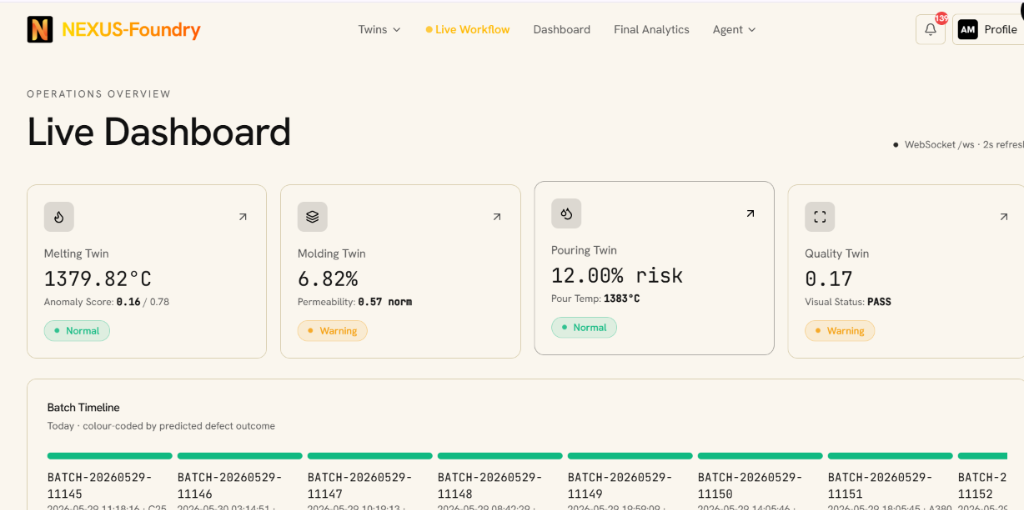
\includegraphics[width=0.48\textwidth]{docs/screenshots/01_live_operations_dashboard.png} \hfill
    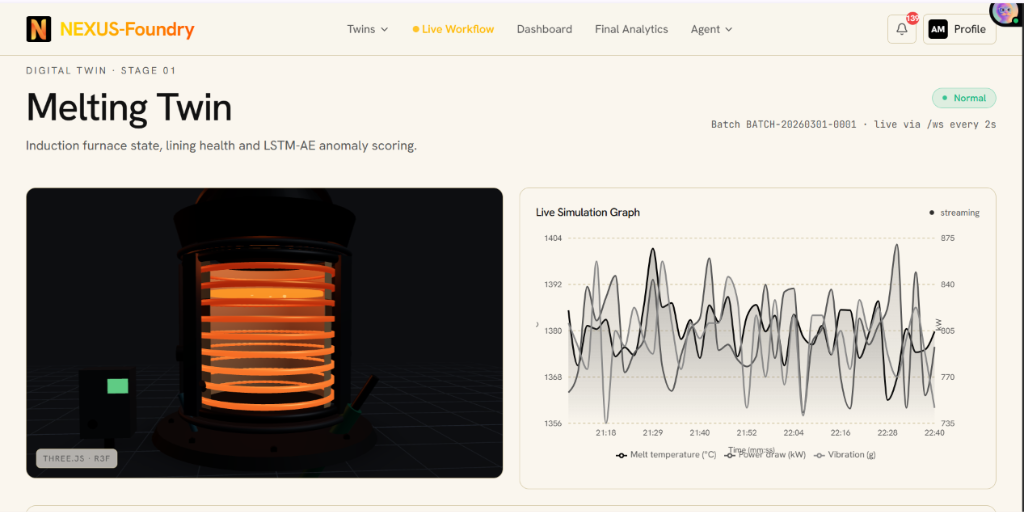
\includegraphics[width=0.48\textwidth]{docs/screenshots/02_melting_twin_3d_simulation.png} \\[0.2cm]
    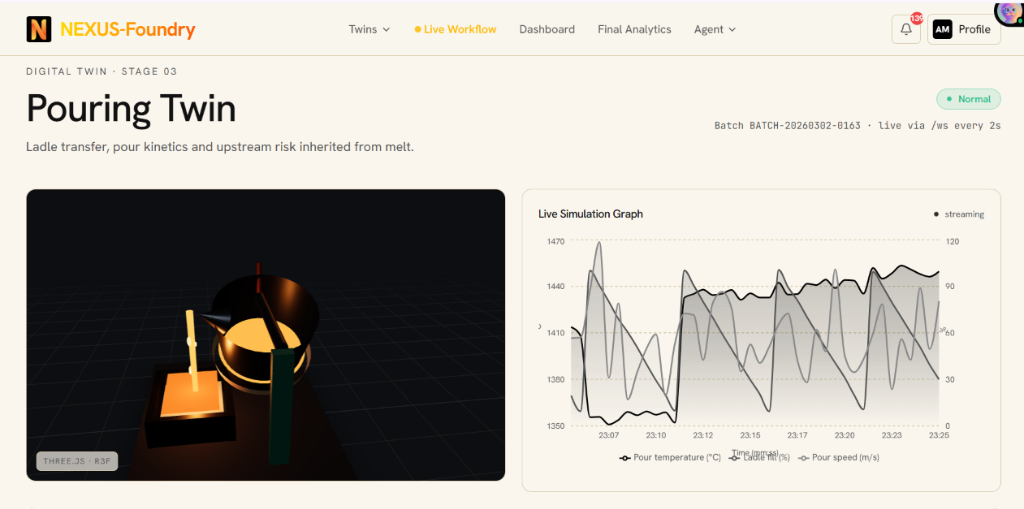
\includegraphics[width=0.48\textwidth]{docs/screenshots/03_pouring_twin_3d_simulation.png} \hfill
    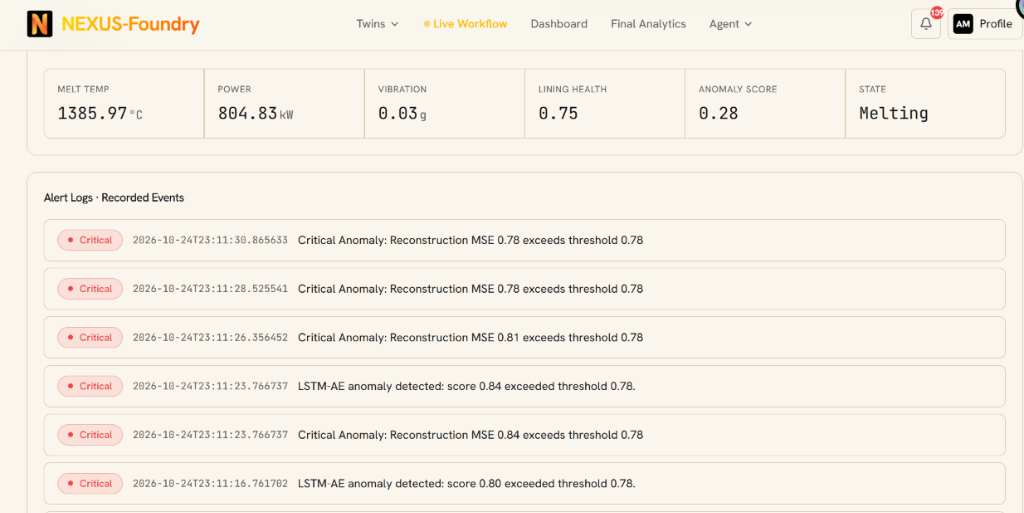
\includegraphics[width=0.48\textwidth]{docs/screenshots/05_critical_alerts_and_anomaly_logs.png}
    \caption{Integrated Software System Demonstration: (Top-Left) Operations Dashboard \& Batch Timeline; (Top-Right) Melting Twin 3D Induction Furnace; (Bottom-Left) Pouring Twin 3D Ladle Pouring; (Bottom-Right) Critical Alerts \& Diagnostics Log}
\end{figure}

% --- 6. TECHNICAL KNOWLEDGE & ENGINEERING DECISIONS ---
\section{Software Engineering Decisions \& Technical Justification}
\begin{itemize}[noitemsep, topsep=2pt]
    \item \textbf{Architectural \& Design Patterns:} The platform adopts an \textit{Event-Driven Microservices Architecture} with strict decoupling of ``memory'' (digital twins managing state) from ``intelligence'' (stateless ML inference engines). The \textit{Observer Pattern} governs real-time WebSocket state broadcasting, while the \textit{Strategy Pattern} encapsulates multi-model predictive execution, allowing individual models to be updated or swapped without disrupting twin operations.
    \item \textbf{Concurrency, Data Integrity \& Security:} High-frequency sensor ingestion is handled via Python's non-blocking \texttt{asyncio} event loop and asynchronous database drivers (\texttt{asyncpg}, \texttt{aiokafka}), ensuring sub-35ms response times. Ephemeral state consistency is maintained through Redis optimistic locking. Proprietary metallurgical recipes and telemetry are secured by enforcing 100\% on-premise model execution (local Llama 3 via Ollama) without external API dependencies.
    \item \textbf{Error Handling, Logging \& Maintainability:} Strict type safety and input sanitization are enforced across all API endpoints using Pydantic v2 schemas. Structured JSON logging enables end-to-end event tracing from MQTT ingress to WebSocket delivery. Automatic graceful fallbacks to calibrated empirical baselines ensure continuous operation even during sensor dropouts.
\end{itemize}

% --- 7. CONCLUSION, LIMITATIONS & FUTURE SCOPE ---
\section{Conclusion, Limitations \& Future Scope}
\begin{itemize}[noitemsep, topsep=2pt]
    \item \textbf{Conclusion:} Phase II has successfully delivered a fully integrated (100\%), cross-stage cyber-physical digital twin platform for smart foundry operations. The system eliminates decoupled process silos by interconnecting melting, molding, pouring, and quality inspection, achieving sub-2.0s anomaly propagation, 48-hour degradation forecasting, and pre-pour defect prevention.
    \item \textbf{Known Limitations:} Optical emission spectrometry (OES) chemical validation currently exhibits a 15--30 minute lab delay, necessitating synthetic interpolation for real-time carbon equivalent calculations. Physical PLC hardware-in-the-loop actuation remains bounded by industrial safety regulations.
    \item \textbf{Future Roadmap:} Phase III will focus on deploying direct hardware integration via industrial OPC-UA / Modbus TCP protocols, closed-loop automated PLC induction power trimming, and multi-tenant cloud scaling across federated foundry clusters.
\end{itemize}

% --- 8. DELIVERABLES & TECHNICAL ENRICHMENT SUMMARY ---
\section{Project Deliverables \& Technical Enrichment Summary}
\begin{table}[H]
    \centering
    \footnotesize
    \renewcommand{\arraystretch}{1.2}
    \begin{tabular}{|p{4.2cm}|p{7.5cm}|c|}
        \hline
        \textbf{Deliverable Category} & \textbf{Details / Title / Repository Link} & \textbf{Status} \\
        \hline
        Source Code Repository & \url{https://github.com/NEXUSFoundry-Your-Foundry-Optimizer/Nexus-Foundry-Platform} & Completed \\
        \hline
        Individual Online Certifications & 
        \textbf{Subiksha M.V}: Digital Twins Explained (Digital Twins in Industry 4.0), Udemy (17.5 hrs) \newline
        \textbf{C.B. Harinie}: Digital Twins Explained (Digital Twins in Industry 4.0), Udemy (17.5 hrs) \newline
        \textbf{K. Kanishthika}: Time Series Analysis and Forecasting with Python, Udemy (10.5 hrs) \newline
        \textbf{P. Pon Gopika}: Time Series Analysis and Forecasting with Python, Udemy (10.5 hrs) & Completed \\
        \hline
        Group TEA Deliverable 1 & Submission-ready Research Paper Draft: \textit{Cross-Stage Cognitive Digital Twin Platform for Predictive Casting Intelligence} & Completed \\
        \hline
        Group TEA Deliverable 2 & Project Website / Interactive Documentation Portal (Live at \url{http://localhost:8081}) & Completed \\
        \hline
        Group TEA Deliverable 3 & Open-source Technical Repository and Calibrated Pyrometallurgical Datasets & Completed \\
        \hline
    \end{tabular}
    \caption{Summary of Completed Project and Technical Enrichment Deliverables}
\end{table}

% --- REFERENCES ---
\vspace{0.2cm}
\nocite{*}
\renewcommand{\refname}{\large\bfseries\color{amritaMaroon}References}
\bibliographystyle{ieeetr}
\bibliography{ref}

\end{document}
